\documentclass{homework}

\title{02MECH - Midterm I \\ 07.11.2022}
%\author{I. Yalcinkaya}

\date{\vspace{-11ex}}

\begin{document}

\maketitle

\exercise
\begin{center}
\textit{``All things in our universe are constantly in motion, vibrating!''}
\end{center}

\begin{figure}[h]
\centering
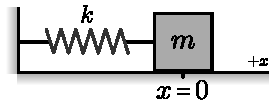
\includegraphics[scale=1]{figures/ho.pdf}
\end{figure}

A block is attached to the wall with a spring as it is shown in the figure. $k$ is the spring constant, $m$ is the mass of the body and $x=0$ is the equilibrium point of the system. It is given that the spring and all connection equipment are massless and the system is completely frictionless. We further assume that no gravitational force is applied on the block and we will only consider very small oscillations so that $x\ll 1$.
\begin{itemize}
    \item [\textbf{(a)}] Sketch the free-body diagrams of the block for $x>0$, $x=0$ and $x<0$.
    \item[\textbf{(b)}] Write down the equation of the motion of the block in differential equation form but do not solve it. Make the suitable substitution for the angular frequency $\omega_0$.
    \item[\textbf{(c)}] By using the solution assumption $x(t)=e^{\lambda t}$ solve the equation of motion in \textbf{(b)} and write down the solution in $x(t)=Ae^{-i\omega_0 t}+Be^{i\omega_0 t}$ form, where $A$ and $B$ are some arbitrary constants.
    \item[\textbf{(d)}] We know that the equation $x(t)=Ae^{-i\omega_0 t}+Be^{i\omega_0 t}$ can be written in $x(t)=C\cos{\left(\omega_o t\right)}$ form (where $C$ is an arbitrary real constant) describing the block's position with respect to time. Determine $C$ for the  initial condition $x(0)=x_0$ describing the initial position of the block at time $t=0$.
    \item[\textbf{(e)}] Let us assume that there is a resisting force in the medium that block moves. The magnitude of the resisting force is proportional to the block's velocity such as $F_f=-b\dot{x}$ where $b$ is the constant of resisting force. Write down the equation of motion of the block in the differential equation form by making substitutions for $\beta=b/2m$ and the natural angular frequency $\omega_0$. Do not solve the differential equation.
    \item[\textbf{(f)}] Given that the solution of the differential equation in \textbf{(e)} is $x(t)=e^{-\beta t}x_0\cos{\left(\omega_1 t\right)}$, how long does it take for the damped oscillator to halve the amplitude of the oscillation? (Givens: $\ln2\approx 0.7$, $m=~1\text{kg}$, $b=1.4~\text{kg/s}$)
    \item[\textbf{(g)}] How many times does the damped oscillator oscillate until it's amplitude is halved (Given: $\pi\approx 3$, $k=1.3~\text{kg/s$^2$}$)? 
\end{itemize}

\textit{Each option is worth 0.2 points - Total: 1.4 points} 

\exercise
\begin{center}
\textit{``Why walking in the rain is not painful?''}
\end{center}

\begin{figure}[h]
\centering
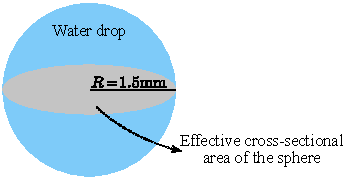
\includegraphics[scale=1.3]{figures/rd.pdf}
\end{figure}

The magnitude of the drag force $D$ in the air is related to an object's relative speed $\nu$ with respect to the air as
\begin{equation*}
    D=\frac{1}{2}C\rho_a A \nu^2,
\end{equation*}
where $\rho_a$ is the air density (mass per volume) and $A$ is the effective cross-sectional area of the body (the area of a cross section taken perpendicular to the velocity). The drag coefficient $C$ is determined experimentally, and it will be assumed that it is a constant for simplicity.

A raindrop initially at rest with radius $R=1.5$ mm falls from a cloud that is height $h=1000$ m above the ground. The drag coefficient $C$ for the drop is $0.80$. Assume that the drop is spherical throughout its fall as it is shown in the figure. The density of water $\rho_w$ is $1000~\text{kg}/\text{m}^3$, and the density of the air is $\rho_a$ is $1.0~\text{kg}/\text{m}^3$. 
\begin{itemize}
    \item[\textbf{(a)}] Write down the gravitational force acting on the raindrop in terms of the parameters $\rho_w$, $R$ and $g$, where $g$ is the gravitational acceleration (Do not calculate it's numerical value).
    \item[\textbf{(b)}] Write down Newton's 2nd law for the raindrop when it reaches its terminal speed in terms of the parameters $D$, $m$ and $g$.
    \item[\textbf{(c)}] By making use of your findings in \textbf{(a)} and \textbf{(b)}, write down the expression giving the raindrop's terminal speed in terms of the parameters $\rho_w$, $\rho_a$, $R$, $g$ and $C$.
    \item[\textbf{(d)}] Calculate the numerical value of the terminal speed of the raindrop in km/h  (Givens: $g\approx 10~\text{m/s}^2$, $\sqrt{50}\approx 7$).
    \item[\textbf{(e)}] What would be the raindrop's speed in km/h just before impact if there were no drag force? (Given: $v=\sqrt{2gh}$ where $v$ is the impact speed of a particle in a gravitational field after it was released from a height $h$, $\sqrt{2}\approx 1.4$).
\end{itemize}

\textit{Each option is worth 0.2 points - Total: 1 point} 

\exercise
\begin{center}
\textit{``Energy can neither be created nor destroyed - only converted from one form to another.''}
\end{center}

\begin{figure}[h]
\centering
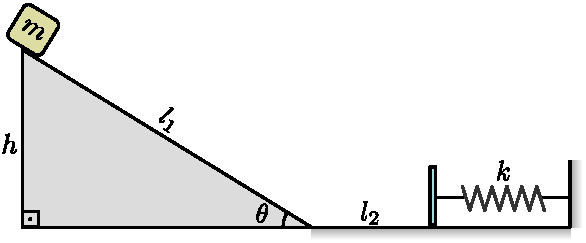
\includegraphics[scale=1]{figures/en.pdf}
\end{figure}

A block of mass $m$ which is initially at rest, is released from the top of a frictionless inclined plane. Under the effect of the gravitational force it covers the distances $l_1$ (length of the inclined surface) and $l_2$ (length from the end of the inclined surface to the equilibrium point of the spring) and compresses a spring with the spring constant $k$. We assume that the spring and the bumper attached to it are massless and frictionless.

\begin{itemize}
    \item[\textbf{(a)}] Express the maximum compression distance in the spring in terms of $m$, $g$, $\theta$, $l_1$ and $k$ if there is no friction in the whole system ($g$ is the gravitational acceleration). 
    \item[\textbf{(b)}] Consider the motion of the block after it compresses the spring maximally. Can the block reach up to height $h$ on it's way back on the inclined plane? Why? Explain it briefly in terms of the conversion energy from one form to another, by words or formulas.
    \item[\textbf{(c)}] Now consider that there is a dry friction between the block and the horizontal surface where the spring system lies (the inclined surface is still frictionless) with a kinetic friction coefficient $\mu_k$. Write down the magnitude of the kinetic friction force $F_f$ between the block and the surface in terms of $\mu_k$, $m$ and $g$.
    \item[\textbf{(d)}] How much work $W$ is done on the block by the frictional force as the block covers the distance $l_2$? Express your result in terms of $\mu_k$, $m$ and $g$ and $l_2$.
    \item[\textbf{(e)}] Express the maximum compression distance of the spring in terms of $\mu_k$, $m$ and $g$, $k$, $l_1$, $l_2$ and $\theta$ (Given: The solution for the quadratic equation $Ax^2+Bx+C=0$ is $x_{1,2}=\left(-B\pm\sqrt{B^2-4AC}\right)/2A$).
    \item[\textbf{(f)}] When we consider the block's motion after it compresses the spring maximally in case of dry friction, can it reach up to height $h$ on it's way back on the inclined plane? Why? Explain it briefly in terms of the conversion energy from one form to another by words or formulas and write down the total mechanical energy loss after the block returns to the inclined plane in terms of $\mu_k$, $m$, $g$, $l_2$ and $x_m$.
\end{itemize}

\textit{Each option is worth 0.2 points - Total: 1.2 points} 

\exercise
\begin{center}
\textit{``When there is no net external force acting on a system of particles the total momentum of the system is conserved.''}
\end{center}

\begin{figure}[h]
\centering
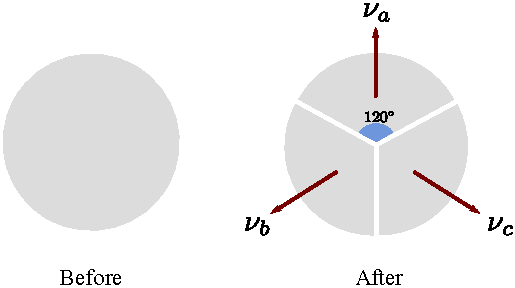
\includegraphics[scale=1]{figures/lm.pdf}
\end{figure}

A disk which is in rest in the beginning is disintegrated into three completely equal pieces as it is shown in the figure. Each mass has the same mass $m$. We are given that $\nu_a$, $\nu_b$, $\nu_c$ are the velocities of the pieces after disintegration and $\nu_a=2~\text{m/s}$. 

\begin{itemize}
    \item[\textbf{(a)}] Sketch the momentum vectors of the pieces, $p_a$, $p_b$, $p_c$, on the same graph and determine the angles between them.
    \item[\textbf{(b)}] Find a relationship between $\nu_b$ and $\nu_c$ by taking into account that the momentum is conserved in $x-$direction.
    \item[\textbf{(c)}] Find a relationship between $\nu_a$, $\nu_b$ and $\nu_c$ by taking into account that the momentum is conserved in $y-$direction.
    \item[\textbf{(d)}] Depending on the results obtained above, calculate the numerical values of $\nu_b$ and $\nu_c$ (Given: $\sin 30^\circ = 1/2$).
\end{itemize}

\textit{Each option is worth 0.25 points - Total: 1 point} 

\end{document}
